\documentclass[aspectratio=169]{beamer}

% ---------- THEME & LOOK ----------
\usetheme{Madrid}
\usecolortheme{seahorse}
\usefonttheme{professionalfonts}
\setbeamertemplate{navigation symbols}{}
\setbeamercovered{transparent}
\setbeamertemplate{itemize items}[circle]
\setbeamertemplate{enumerate items}[default]
\setlength{\parskip}{0.25em}

% ---------- COLORS ----------
\usepackage{xcolor}
\definecolor{accent}{RGB}{0,92,184}
\definecolor{soft}{RGB}{233,244,255}
\setbeamercolor{structure}{fg=accent}
\setbeamercolor{title}{fg=white,bg=accent}
\setbeamercolor{frametitle}{fg=accent}
\setbeamercolor{block title}{bg=accent!10,fg=accent}
\setbeamercolor{block body}{bg=soft}

% ---------- PACKAGES ----------
\usepackage{booktabs}
\usepackage{amsmath, amssymb}
\usepackage{array}
\usepackage{graphicx}
\usepackage{hyperref}
\hypersetup{colorlinks=true,linkcolor=accent,urlcolor=accent}

% ---------- PLACEHOLDER BOX ----------
\newcommand{\placeholderbox}[2][0.82\linewidth]{%
  \begin{center}
    \fbox{\begin{minipage}[c][0.46\textheight][c]{#1}
      \centering \vspace{0.25em}
      \textbf{#2}\\[0.6em]
      \emph{Insert figure/table here later.}
    \end{minipage}}
  \end{center}
}

% ---------- TITLE ----------
\title{\textbf{Unemployment: Causes and Consequences}}
\subtitle{{\large ECON 300 - Labour Economics}}
\author{Muhebullah Karimzada}
\date{Winter 2026}

\begin{document}

% ============================================================
% TITLE
% ============================================================
\begin{frame}[plain]
  \titlepage
\end{frame}

% ============================================================
\section{Orientation}
% ============================================================

\begin{frame}{Learning Objectives (1/2)}
\transfade
\begin{itemize}
  \item Explain how imperfect information can generate the coexistence of unemployment and vacancies.
  \item Assess how technological change, especially the Internet, affects job search and matching.
  \item Show how demand shifts and sectoral change can generate unemployment.
  \item Summarize evidence on job displacement and its consequences.
\end{itemize}

\end{frame}

\begin{frame}{Learning Objectives (2/2)}
\transfade
\begin{itemize}
  \item Describe models where firms pay above-market wages: efficiency wages, implicit contracts, and insider--outsider models.
  \item Explain the rationale for unemployment insurance/employment insurance and its effects on labour supply and unemployment.
  \item Summarize empirical evidence on UI/EI, incidence, and duration of unemployment.
\end{itemize}


\end{frame}

\begin{frame}{Main Questions}
\transfade
\begin{itemize}
  \item What role does wage rigidity play in unemployment?
  \item How does imperfect information create frictional unemployment?
  \item Is online search improving matching efficiency?
  \item What are the consequences of job loss for workers and families?
  \item Does UI/EI do more harm than good?
\end{itemize}


\end{frame}

% ============================================================
\section{Causes of Unemployment}
% ============================================================

\begin{frame}{Causes of Unemployment}
\transfade
\begin{itemize}
  \item Minimum wage laws
  \item Institutional factors such as unions or a large public sector
  \item Demand factors and seasonal unemployment
  \item Frictional unemployment arising from turnover and imperfect information
  \item Sectoral shifts causing structural unemployment
  \item Generous UI/EI affecting search incentives
\end{itemize}

\begin{block}{Definitions}
\begin{itemize}
  \item \textbf{Frictional unemployment:} short-term unemployment arising from normal job search and turnover.
  \item \textbf{Structural unemployment:} unemployment caused by mismatches between worker skills/locations and available jobs.
  \item \textbf{Seasonal unemployment:} recurring unemployment related to seasonal patterns in industries such as tourism, agriculture, or construction.
\end{itemize}
\end{block}
\end{frame}

\begin{frame}{Interpreting the Different Causes}
\transfade
\begin{itemize}
  \item Not all unemployment has the same cause, so not all unemployment should be addressed with the same policy.
  \item Frictional unemployment may require better information and matching.
  \item Structural unemployment may require retraining or geographic mobility.
  \item Cyclical unemployment may require macroeconomic stimulus.
\end{itemize}

\begin{exampleblock}{Real Example}
A laid-off oil worker in Alberta may face structural unemployment if jobs are growing mainly in healthcare or technology rather than energy.
\end{exampleblock}
\end{frame}

% ============================================================
\section{Search Unemployment}
% ============================================================

\begin{frame}{Search Unemployment: Core Ideas}
\transfade
\begin{itemize}
  \item Imperfect information delays matching between workers and firms.
  \item Searching for jobs has both costs and benefits.
  \item Workers adopt a \textbf{stopping rule} or \textbf{reservation criterion}: accept the first offer that meets a minimum acceptable standard.
  \item Optimal search balances expected marginal benefit and expected marginal cost.
\end{itemize}


\end{frame}

\begin{frame}{Why Search Takes Time}
\transfade
\begin{itemize}
  \item Workers do not observe all vacancies instantly.
  \item Firms do not immediately identify the best applicants.
  \item Search time can improve job match quality, but it also delays income.
\end{itemize}

\begin{block}{Interpretation}
A longer search may be rational if it increases the chance of finding a better job. Unemployment is not always wasteful; some of it is part of efficient job matching.
\end{block}

\begin{exampleblock}{Real Example}
A recent graduate may reject a low-wage unrelated job and search longer for an entry-level job in their field because the long-run payoff is better.
\end{exampleblock}
\end{frame}

\begin{frame}{Figure 17.1: Optimal Job Search}
\centering
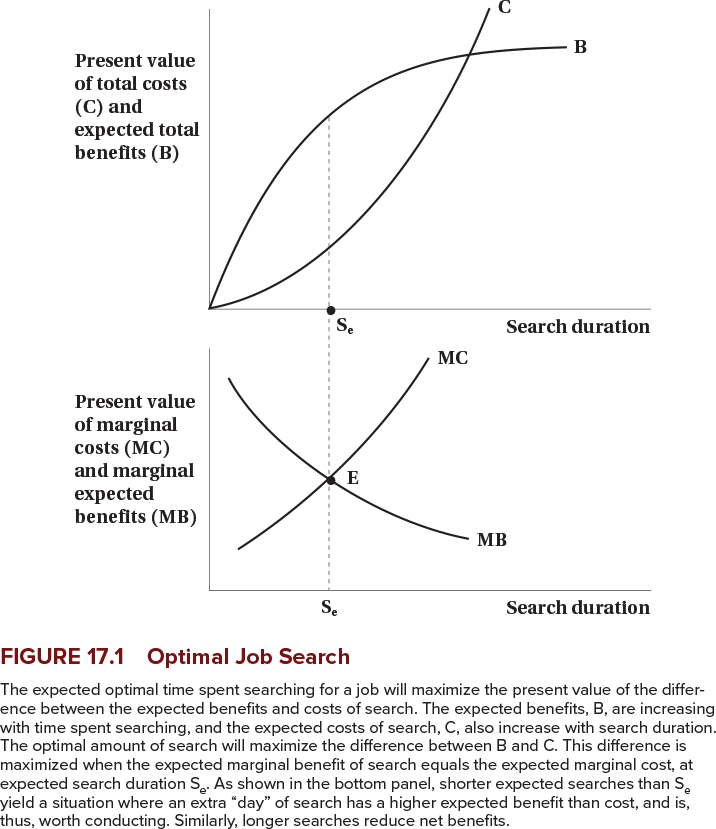
\includegraphics[width=0.55\linewidth]{ben54842_1701}
\end{frame}

\begin{frame}{Reading Figure 17.1}
\transfade
\begin{itemize}
  \item In the top panel, total expected benefits of search rise at first but eventually flatten.
  \item Total costs rise as search continues.
  \item In the bottom panel, optimal search occurs where \textbf{marginal expected benefit equals marginal cost}.
\end{itemize}

\begin{block}{Interpretation}
The optimal search duration is not necessarily zero. It is efficient to keep searching until the extra expected gain from one more unit of search just equals its cost.
\end{block}
\end{frame}

\begin{frame}{Worked Example: Reservation Wage and Hazard}
\transfade
Julia faces three job offers with equal probability: \$2,400, \$2,200, and \$2,000 per month.

\begin{itemize}
  \item Expected value of the next offer:
  \[
  E[W] = \frac{2400 + 2200 + 2000}{3} = 2200
  \]
  \item Reservation wage:
  \[
  W^R = 2200
  \]
  \item She rejects any offer below \$2,200 and accepts the first offer at or above \$2,200.
  \item Acceptance probability:
  \[
  P(W \geq 2200) = \frac{2}{3}
  \]
\end{itemize}

\begin{block}{Definition}
The \textbf{hazard rate} is the probability that an unemployed worker exits unemployment in a given period, conditional on still being unemployed.
\end{block}
\end{frame}

\begin{frame}{Interpreting Reservation Wage}
\transfade
\begin{itemize}
  \item Higher search cost lowers the reservation wage.
  \item Better future offer prospects raise the reservation wage.
  \item Higher unemployment benefits may allow workers to search longer and hold out for better jobs.
\end{itemize}

\begin{exampleblock}{Real Example}
A worker with savings or EI benefits may reject a very low offer and continue searching, while a worker with no buffer may accept quickly.
\end{exampleblock}
\end{frame}


% ============================================================
\section{Imperfect Information}
% ============================================================

\begin{frame}{Imperfect Information: Market Implications}
\transfade
\begin{itemize}
  \item Markets do not clear instantaneously.
  \item Wage dispersion can persist even with homogeneous workers and jobs.
  \item Individual firms may face upward-sloping labour supply because search frictions reduce worker mobility.
\end{itemize}

\begin{block}{Definition}
\textbf{Dynamic monopsony} refers to a setting where individual firms have some wage-setting power because workers face frictions in moving between jobs.
\end{block}
\end{frame}

\begin{frame}{Why Wage Dispersion Can Persist}
\transfade
\begin{itemize}
  \item If workers do not observe all wages, some firms can pay less and still attract workers.
  \item Search frictions prevent immediate movement to the best-paying employer.
  \item This helps explain why similar workers may earn different wages in similar jobs.
\end{itemize}

\begin{exampleblock}{Real Example}
Two retail firms in the same city may pay different wages because workers do not instantly know all job offers and switching jobs is costly.
\end{exampleblock}
\end{frame}

\begin{frame}{Figure 17.2: Wage Distributions Under Imperfect vs. Perfect Information}
\centering
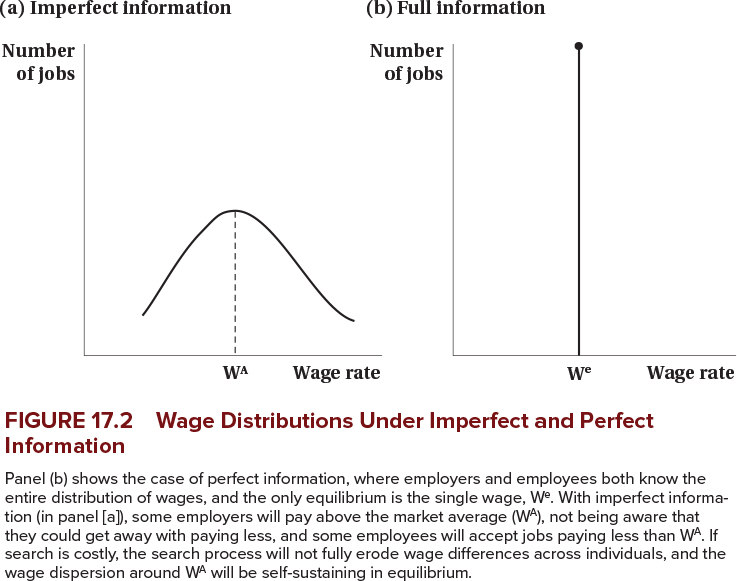
\includegraphics[width=0.89\linewidth]{ben54842_1702}
\end{frame}

\begin{frame}{Reading Figure 17.2}
\transfade
\begin{itemize}
  \item Under imperfect information, wages are spread over a distribution.
  \item Under full information, wages collapse to a single market-clearing wage.
\end{itemize}

\begin{block}{Interpretation}
Search frictions help explain both unemployment and persistent wage differences. Without frictions, workers would all move immediately to the highest available wage and wage dispersion would disappear.
\end{block}
\end{frame}

% ============================================================
\section{Search, Internet, and Matching}
% ============================================================

\begin{frame}{Search, the Internet, and Matching}
\transfade
\begin{itemize}
  \item Online job boards, employer portals, and screening tools have grown rapidly.
  \item Technology can raise contact rates between workers and firms.
  \item Better screening may improve match quality and shorten vacancy duration.
\end{itemize}

\begin{block}{Interpretation}
Technology may reduce frictional unemployment by lowering search costs, but it can also raise application volume and screening complexity for employers.
\end{block}
\end{frame}

\begin{frame}{Has Online Search Solved Search Frictions?}
\transfade
\begin{itemize}
  \item It often makes vacancy information easier to access.
  \item But search is still imperfect:
  \begin{itemize}
    \item workers may not know which applications are worth sending,
    \item firms may struggle to process many applications,
    \item online systems may filter out qualified candidates.
  \end{itemize}
\end{itemize}

\begin{exampleblock}{Real Example}
A worker can apply to 200 jobs online in a week, but still remain unemployed if applications are poorly targeted or automated filters reject them.
\end{exampleblock}
\end{frame}

% ============================================================
\section{Sectoral Shifts}
% ============================================================

\begin{frame}{Sectoral Shifts and Unemployment}
\transfade
\begin{itemize}
  \item Major structural change raises unemployment during reallocation.
  \item Highly cyclical industries amplify unemployment in downturns.
  \item Regional reallocation in Canada drives migration, retraining, and search.
\end{itemize}

\begin{block}{Definition}
\textbf{Sectoral shifts} are changes in the pattern of labour demand across industries or regions.
\end{block}
\end{frame}

\begin{frame}{Why Sectoral Shifts Create Unemployment}
\transfade
\begin{itemize}
  \item Workers displaced from shrinking sectors do not automatically match into expanding ones.
  \item Skills may not transfer perfectly.
  \item Geography matters if jobs grow in different provinces or cities.
\end{itemize}

\begin{exampleblock}{Real Example}
A decline in manufacturing may reduce jobs in one region while healthcare and technology jobs expand elsewhere. Workers may need retraining or relocation to re-enter employment.
\end{exampleblock}
\end{frame}

\begin{frame}{Figure 17.3: Regional Unemployment Rates, 1976--2019}
\centering
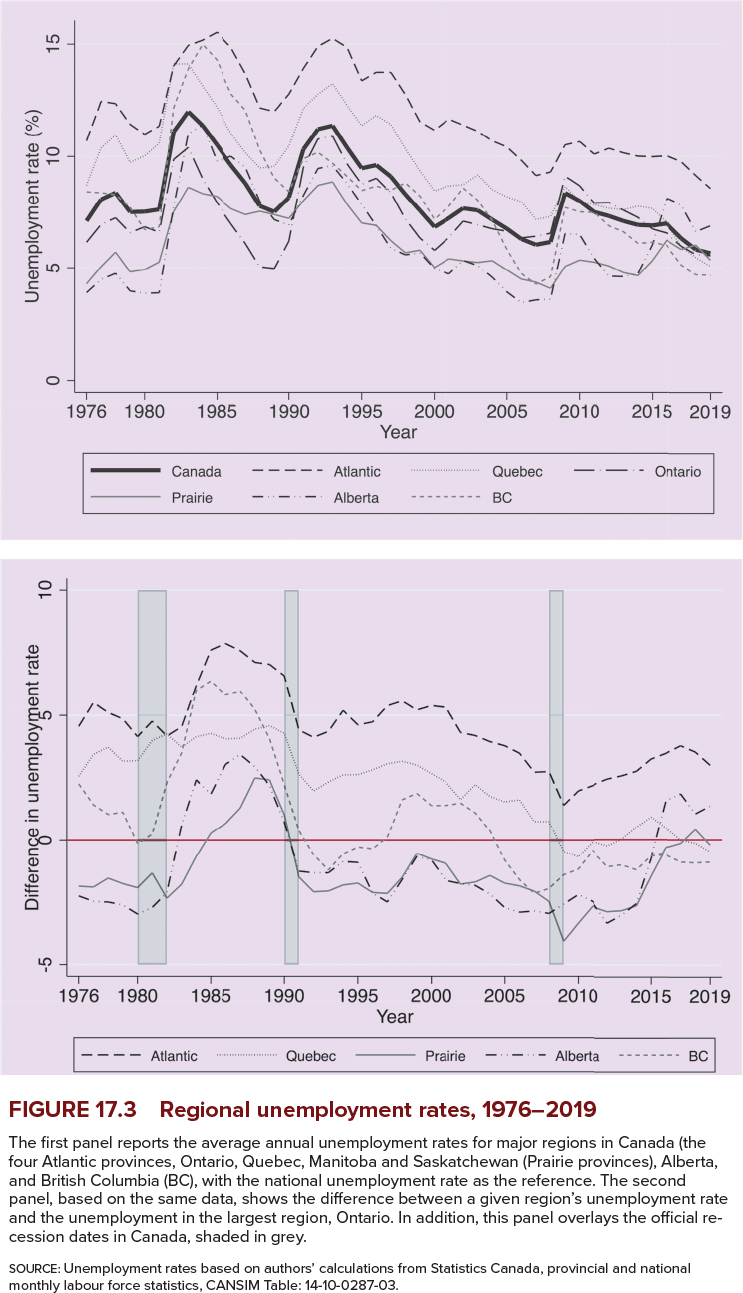
\includegraphics[width=0.7\linewidth]{ben54842_1703}
\end{frame}

\begin{frame}{Reading Figure 17.3}
\transfade
\begin{itemize}
  \item Regional unemployment rates in Canada differ persistently.
  \item Some provinces face chronically higher unemployment than others.
  \item Regional shocks do not disappear instantly because moving is costly and local industry structures differ.
\end{itemize}

\begin{block}{Interpretation}
Regional unemployment differences suggest that labour markets are not perfectly integrated. Geography is an important part of structural unemployment.
\end{block}
\end{frame}

% ============================================================
\section{Displaced Workers}
% ============================================================

\begin{frame}{Displaced Workers: Stylized Findings}
\transfade
\begin{itemize}
  \item Permanent job loss often causes large earnings losses.
  \item Re-employment frequently occurs at substantially lower wages.
  \item Losses can persist for many years.
  \item Older and less-educated workers often have lower re-employment probabilities.
\end{itemize}

\begin{block}{Definition}
\textbf{Job displacement} refers to involuntary job loss due to reasons such as plant closure, downsizing, or restructuring.
\end{block}
\end{frame}

\begin{frame}{Consequences of Job Displacement}
\transfade
\begin{itemize}
  \item Lower future wages
  \item Longer unemployment spells
  \item Loss of firm-specific human capital
  \item Stress on family well-being and mental health
\end{itemize}

\begin{exampleblock}{Real Example}
A worker laid off after 20 years in a unionized manufacturing plant may eventually find work, but at a lower wage and with weaker benefits in a different sector.
\end{exampleblock}
\end{frame}

% ============================================================
\section{Wage Rigidity Approaches}
% ============================================================

\begin{frame}{Three Approaches}
\transfade
\begin{itemize}
  \item \textbf{Implicit contracts:} risk sharing, rigid wages, layoffs in bad states.
  \item \textbf{Efficiency wages:} firms pay above-market wages to raise productivity or reduce turnover.
  \item \textbf{Insider--outsider theory:} incumbents influence bargaining while outsiders have little influence.
\end{itemize}

\begin{block}{Interpretation}
All three models help explain why wages may stay above market-clearing levels, generating persistent unemployment.
\end{block}
\end{frame}

\begin{frame}{Implicit Contracts: Risk Sharing}
\transfade
\begin{itemize}
  \item Workers are often more risk-averse than firms because their human capital is not easily diversified.
  \item Firms may offer relatively stable wages across states of nature.
  \item Employment adjusts instead of wages, especially in bad states.
\end{itemize}

\begin{block}{Definition}
An \textbf{implicit contract} is an informal or self-enforcing arrangement where firms smooth wages in exchange for flexibility in employment.
\end{block}
\end{frame}

\begin{frame}{Figure 17.4: Implicit Contracts}
\centering
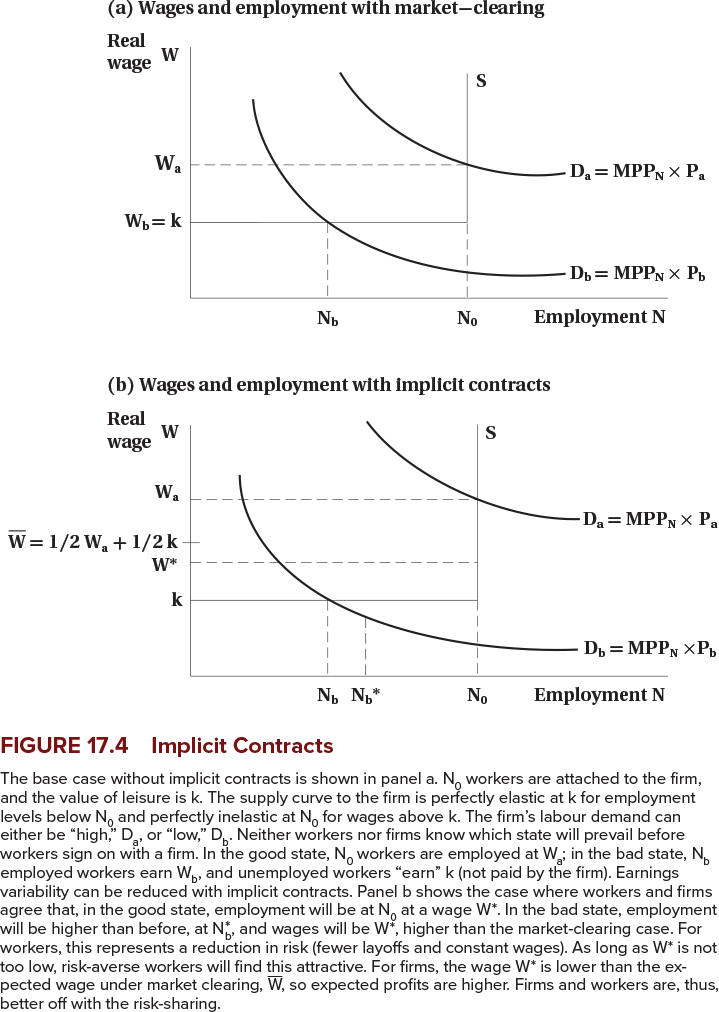
\includegraphics[width=0.485\linewidth]{ben54842_1704}
\end{frame}

\begin{frame}{Reading Figure 17.4}
\transfade
\begin{itemize}
  \item In a market-clearing world, wages fluctuate with labour demand.
  \item Under implicit contracts, wages are smoother.
  \item Employment absorbs more of the adjustment in bad states.
\end{itemize}

\begin{block}{Interpretation}
Risk sharing can make workers better off ex ante, but it can also create layoffs and unemployment when demand is weak.
\end{block}
\end{frame}

\begin{frame}{Efficiency Wages: Core Mechanisms}
\transfade
\begin{itemize}
  \item Higher wages may raise morale and effort.
  \item Higher wages may reduce shirking and turnover.
  \item Firms may use high wages to deter unionization or attract better applicants.
  \item In some models, better nutrition also raises productivity at low wage levels.
\end{itemize}

\begin{block}{Definition}
An \textbf{efficiency wage} is a wage deliberately set above the market-clearing wage because it improves worker productivity or lowers labour costs through other channels.
\end{block}
\end{frame}

\begin{frame}{Figure 17.5: Determination of the Efficiency Wage}
\centering
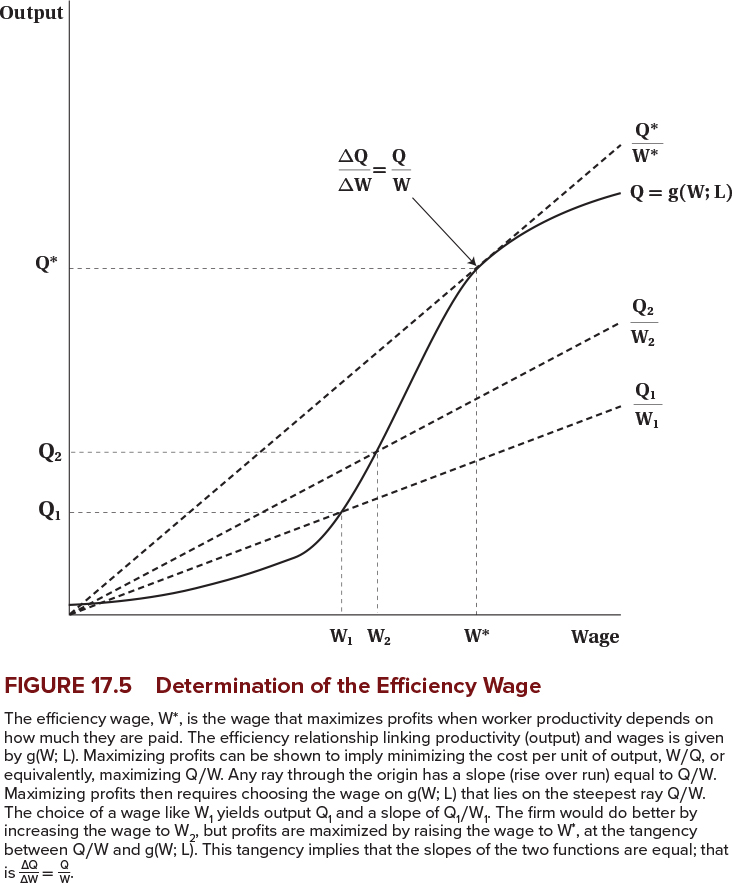
\includegraphics[width=0.54\linewidth]{ben54842_1705}
\end{frame}

\begin{frame}{Reading Figure 17.5}
\transfade
\begin{itemize}
  \item Output rises with the wage because worker efficiency increases.
  \item But the gain from raising the wage eventually diminishes.
  \item The optimal efficiency wage is where the gain from better performance is balanced against the higher wage cost.
\end{itemize}

\begin{block}{Interpretation}
If firms pay efficiency wages, unemployment can persist because wages stay above the level that would clear the labour market.
\end{block}
\end{frame}

\begin{frame}{Insider--Outsider Theory}
\transfade
\begin{itemize}
  \item Wages are bargained mainly with incumbent workers.
  \item Replacing insiders with outsiders is costly because of hiring, training, and disruption costs.
  \item Excess labour supply from outsiders may not push wages down much.
\end{itemize}

\begin{block}{Definition}
\textbf{Insiders} are current employees with bargaining power. \textbf{Outsiders} are unemployed or non-employed workers who want jobs but have little influence on wage setting.
\end{block}
\end{frame}

\begin{frame}{Why Insider--Outsider Forces Matter}
\transfade
\begin{itemize}
  \item Firms may prefer to keep current workers at high wages rather than replace them.
  \item This can generate wage rigidity and persistent unemployment.
  \item Outsiders may remain unemployed even if they are willing to work for less.
\end{itemize}

\begin{exampleblock}{Real Example}
A firm may keep experienced employees at negotiated wages because replacing them would require costly training and risk production disruptions.
\end{exampleblock}
\end{frame}

% ============================================================
\section{UI / EI}
% ============================================================

\begin{frame}{Economic Rationale for UI/EI}
\transfade
\begin{itemize}
  \item UI/EI provides insurance against income loss from unemployment.
  \item It also affects incidence and duration of unemployment through incentives and liquidity.
\end{itemize}

\begin{block}{Definition}
\textbf{Unemployment Insurance (UI)} or \textbf{Employment Insurance (EI)} is a social insurance program that partially replaces lost earnings for eligible unemployed workers.
\end{block}
\end{frame}

\begin{frame}{Why Have UI/EI?}
\transfade
\begin{itemize}
  \item Workers cannot fully insure themselves against job loss.
  \item Private insurance markets may fail because job loss risk is correlated across workers during recessions.
  \item Social insurance smooths consumption and reduces hardship.
\end{itemize}

\begin{exampleblock}{Real Example}
A worker laid off in a recession may have mortgage or rent payments due immediately. EI helps smooth income while they search for a new job.
\end{exampleblock}
\end{frame}

\begin{frame}{Channels: Incidence and Duration}
\transfade
\begin{itemize}
  \item Higher benefits may increase separations by making unemployment less costly.
  \item For unemployed workers, higher benefits lower search costs and may lengthen optimal search.
  \item Empirically, exit rates often rise sharply as benefits approach exhaustion.
\end{itemize}

\begin{block}{Interpretation}
UI/EI creates a trade-off: it provides valuable insurance but may also increase unemployment by affecting job separation and job search behaviour.
\end{block}
\end{frame}

\begin{frame}{Canada's UI/EI System: Key Features}
\transfade
\begin{itemize}
  \item Established in 1940.
  \item Major reforms in 1971--72.
  \item Renamed Employment Insurance in 1996.
  \item Replacement rate around 55\% for beneficiaries.
  \item Claimant types include frequent, long-tenured, and occasional users.
\end{itemize}

\begin{block}{Interpretation}
The details of eligibility and benefit duration matter greatly for how EI affects both insurance value and labour market incentives.
\end{block}
\end{frame}

\begin{frame}{Behavioural Effects and Design Considerations}
\transfade
\begin{itemize}
  \item Moral hazard vs. liquidity effects
  \item Repeat use and seasonal patterns
  \item Regional extended benefits
  \item Labour force participation effects
\end{itemize}

\begin{block}{Definitions}
\begin{itemize}
  \item \textbf{Moral hazard:} insurance changes behaviour because the insured event becomes less costly.
  \item \textbf{Liquidity effect:} benefits allow workers to avoid accepting poor job matches immediately.
\end{itemize}
\end{block}
\end{frame}

\begin{frame}{Interpreting the EI Design Trade-Off}
\transfade
\begin{itemize}
  \item A well-designed system should protect workers from hardship.
  \item But it should also preserve incentives for efficient job search and employment.
  \item The optimal design balances social insurance against induced unemployment.
\end{itemize}

\begin{exampleblock}{Real Example}
If EI is too stingy, workers may be forced into poor matches quickly. If it is too generous for too long, some may delay search excessively. Good design tries to avoid both extremes.
\end{exampleblock}
\end{frame}

% ============================================================
\section{Summary}
% ============================================================

\begin{frame}{Summary}
\transfade
\begin{itemize}
  \item Wage rigidity and imperfect information explain how unemployment can coexist with vacancies.
  \item Search theory uses reservation wages and hazard rates to explain unemployment duration.
  \item Sectoral shifts and job displacement can generate large and persistent costs.
  \item Above-market wages can arise through implicit contracts, efficiency wages, and insider--outsider mechanisms.
  \item UI/EI provides valuable insurance but also affects incidence and duration of unemployment.
\end{itemize}


\end{frame}

\begin{frame}
\centering
\Huge{\textbf{Thank You!}}
\end{frame}

\end{document}